\documentclass[11pt]{beamer}

% use utf8 instead of latin1 when using LaTeX in windows
\usepackage[utf8]{inputenc}

%ds custom packages
%\usepackage{cleveref}
\usepackage{empheq}
\usepackage{graphicx}
\usepackage[font={small}]{caption}
\usepackage{subcaption}
\usepackage{framed}
\usepackage{listings}
\usepackage{wrapfig}
\usepackage{sidecap}
\usepackage{xcolor}
\usepackage{lineno}
\usepackage{marvosym}
\usepackage{xstring}
\usepackage{mfirstuc}
\usepackage{hyperref}
\usepackage{biblatex}

\lstset { %
    language=C++,
    backgroundcolor=\color{black!5}, % set backgroundcolor
    basicstyle=\footnotesize,% basic font setting
}

%ds colors
\definecolor{orange}{rgb}{1,0.4,0}
\definecolor{green}{rgb}{0,0.5,0}

%ds referencing
\newcommand{\myref}[3]{\hyperref[#1]{#2} (\capitalisewords{#3} \ref{#1})}

%ds blue box
\definecolor{myblue}{rgb}{.9, .9, 1}

\newlength\mytemplen
\newsavebox\mytempbox
\newcommand*\widefbox[1]{\fbox{\hspace{2em}#1\hspace{2em}}}

\makeatletter
\newcommand\mybluebox{%
    \@ifnextchar[%]
       {\@mybluebox}%
       {\@mybluebox[0pt]}}

\def\@mybluebox[#1]{%
    \@ifnextchar[%]
       {\@@mybluebox[#1]}%
       {\@@mybluebox[#1][0pt]}}

\def\@@mybluebox[#1][#2]#3{
    \sbox\mytempbox{#3}%
    \mytemplen\ht\mytempbox
    \advance\mytemplen #1\relax
    \ht\mytempbox\mytemplen
    \mytemplen\dp\mytempbox
    \advance\mytemplen #2\relax
    \dp\mytempbox\mytemplen
    \colorbox{myblue}{\hspace{1em}\usebox{\mytempbox}\hspace{1em}}}

%ds global definitions
\def\P{\mathcal P}
\def\tab{\phantom{tab}}
\def\homx{\mathbf{\tilde{x}}}
\def\trans{\mathbf{t}}
\def\quat{\mathbf{q}}
\renewcommand{\thesubfigure}{\arabic{subfigure}}

\renewcommand{\footnotesize}{\tiny}

%ds set background template
\usebackgroundtemplate
{
    
\includegraphics[width=\paperwidth]{figures/slides.pdf}%
}

%ds disable controls on slides
\setbeamertemplate{navigation symbols}{}

%ds info
\title{Online large-scale SLAM with stereo visual-inertial sensors}
\author{Dominik Schlegel}
\date{\today}

%ds redefine footline
\makeatother
\setbeamertemplate{footline}
{
\vspace{5pt}
  \hbox{%
  \hspace{10pt}
  \begin{beamercolorbox}[wd=.7\paperwidth,ht=2.25ex,dp=1ex,center]{author in head/foot}%
    \textcolor{white}{\hspace{70pt}\inserttitle}
  \end{beamercolorbox}%
  \begin{beamercolorbox}[wd=.3\paperwidth,ht=2.25ex,dp=1ex,center]{title in head/foot}%
    \textcolor{white}{\insertdate}\hspace*{3em}
    \textcolor{white}{\insertframenumber{}}\hspace*{1ex}
  \end{beamercolorbox}}%
  \vspace{2pt}%
}
\makeatletter

\begin{document}

%ds titlepage
{
\setbeamertemplate{footline}{} 
\usebackgroundtemplate{
\includegraphics[width=\paperwidth]{figures/titlepage.pdf}}
\begin{frame}
\vspace{-70pt}
\center{\Huge{\textcolor{white}{\inserttitle}}}\\
\vspace{20pt}
\begin{minipage}{1.07\textwidth}
\textcolor{white}{\hfill\small{\insertauthor}}\\
\textcolor{white}{\hfill\small{Supervisor: Prof. Dr. Giorgio Grisetti}}
\end{minipage}
\vspace{10pt}\\
\hspace{-28pt}\textcolor{white}{\small{\insertdate}}
\end{frame}
}

\setcounter{framenumber}{0}

\begin{frame}{Aim of this project}
Map the world using a stereo camera and an IMU:
\begin{figure}[!htb]
\centering
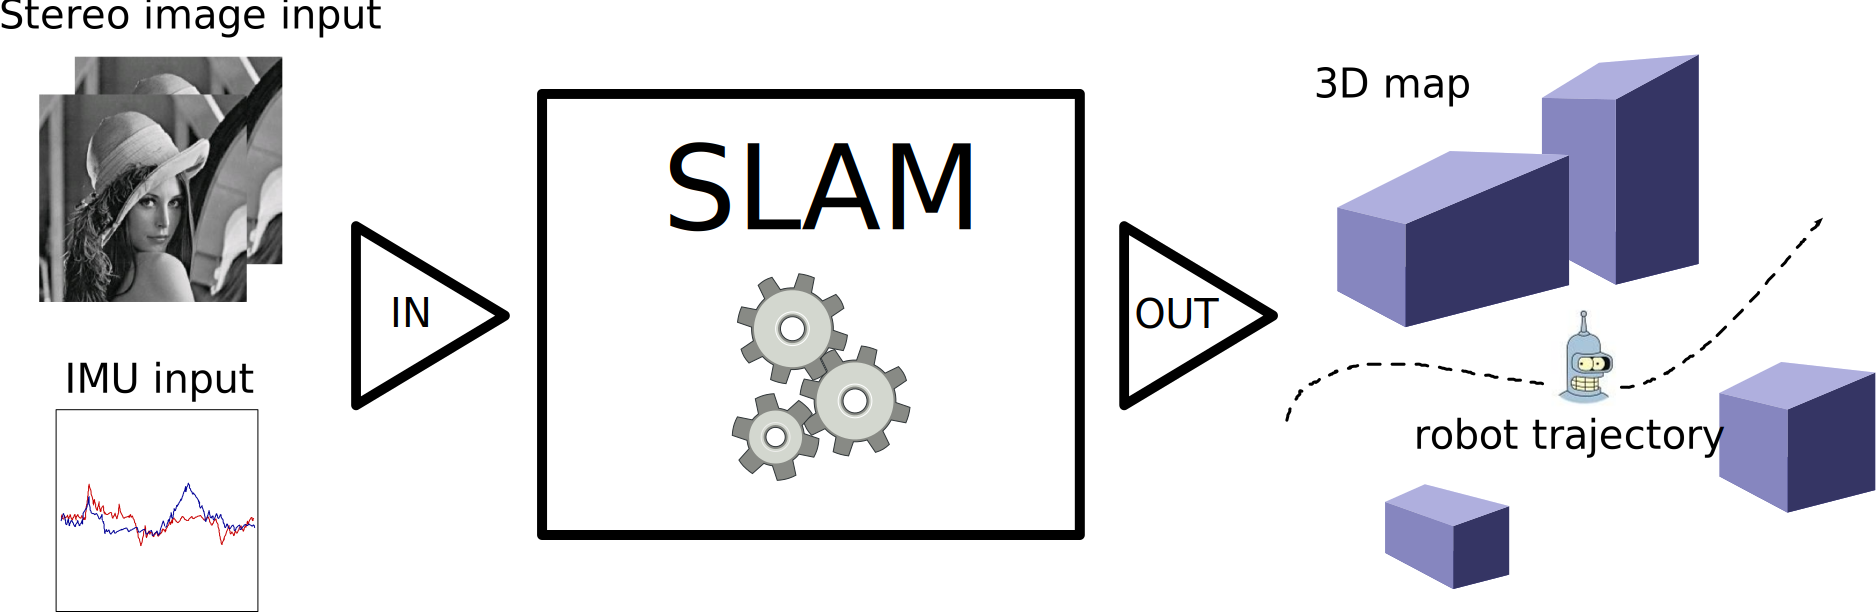
\includegraphics[width=\textwidth]{figures/introduction/basic_concept.pdf}
\end{figure}
Required capabilities:
\begin{itemize}
\item Tracking  (Localization)
\item Mapping (Solving SLAM problem)
\end{itemize}
\end{frame}

\begin{frame}
\frametitle{Graph-based SLAM: The problem}
\begin{figure}[!htb]
\centering
\includegraphics[width=0.9\textwidth]{figures/approach_fundamentals/overview_graphslam_simplified.pdf}
\end{figure}
\vspace{14.9pt}
\end{frame}

\begin{frame}
\frametitle{Graph-based SLAM: The solution with g2o
\footfullcite{Kuemmerle, R., Grisetti, G., Strasdat, H., Konolige, K., Burgard, W.: g2o: A
general framework for graph optimization (ICRA 2011)}}
\begin{figure}[!htb]
\centering
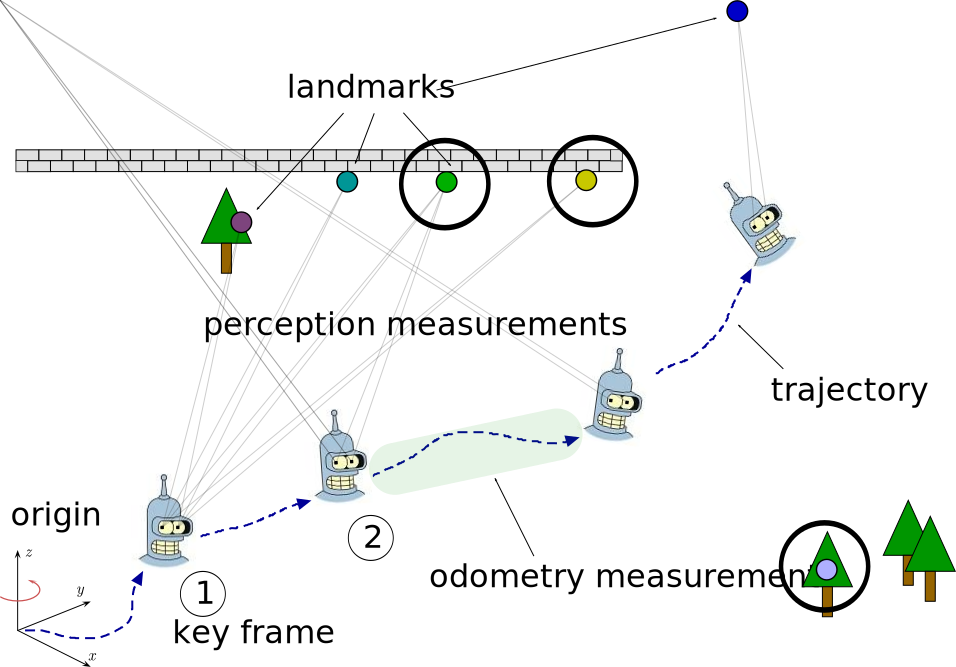
\includegraphics[width=0.9\textwidth]{figures/approach_fundamentals/overview_graphslam_simplified_solved.pdf}
\end{figure}
\end{frame}

\begin{frame}{State of the art}
Google (street) mapping
\begin{figure}[!htb]
\centering
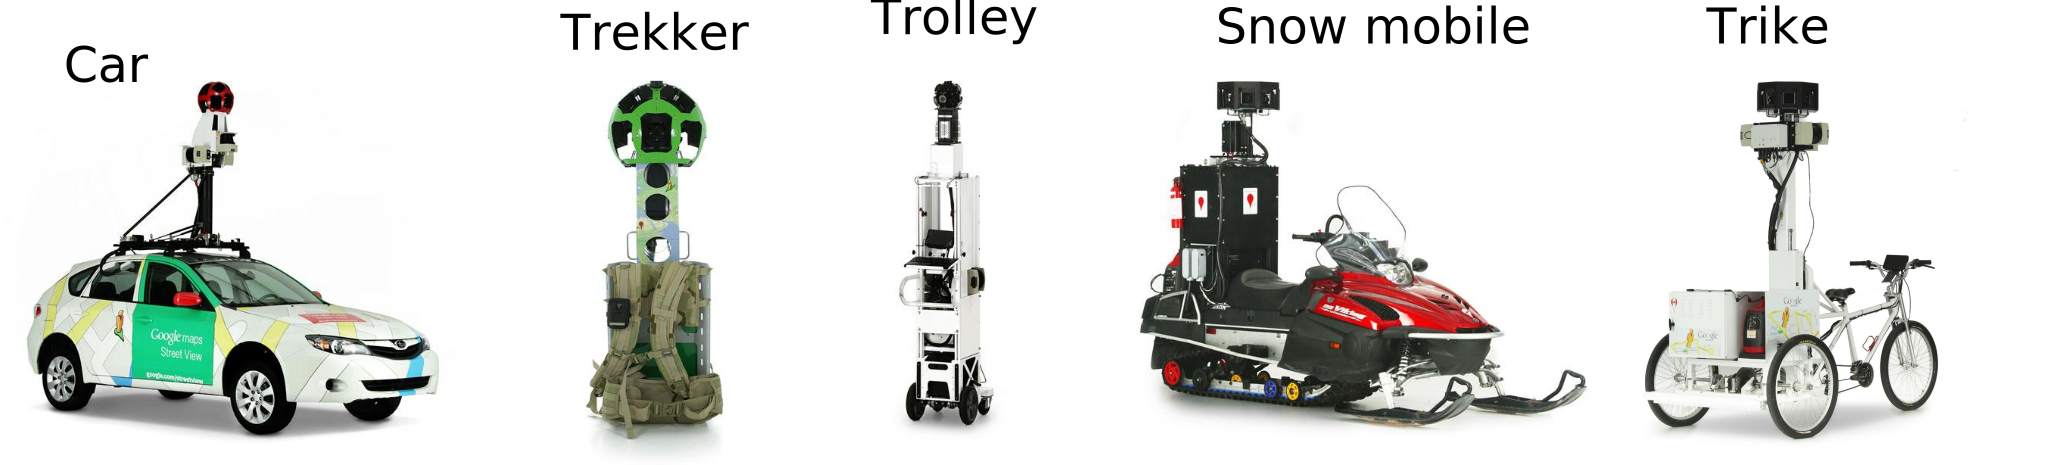
\includegraphics[width=\textwidth]{figures/introduction/google_fleet.pdf}
\vspace{10pt}\\
ORB-SLAM \hspace{15pt} FrameSLAM \hspace{10pt} MonoSLAM \hspace{20pt} SVO\hfill\vspace{5pt}\\
\begin{subfigure}[b]{\textwidth}
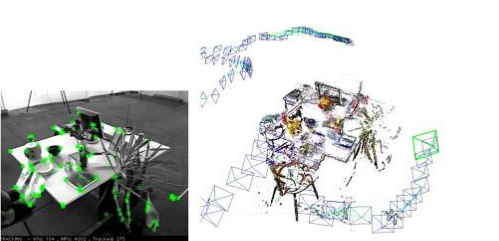
\includegraphics[scale=0.2]{figures/introduction/ORB_SLAM.pdf}
\includegraphics[scale=0.1]{figures/introduction/frameslam.pdf}
\includegraphics[scale=0.1]{figures/introduction/monoslam.pdf}
\includegraphics[scale=0.1]{figures/introduction/svo.pdf}
\end{subfigure}
\end{figure}
\end{frame}

%\footfullcite{Mur-Artal, R., Montiel, J., Tardos, J.D.: ORB-SLAM: a Versatile and Accurate Monocular SLAM System (RSS 2015)}

\begin{frame}{Sensor setup: the VI-Sensor
\footfullcite{Nikolic, J., Rehder, J., Burri, M., Gohl, P., Leutenegger, S., Furgale, P.T., Siegwart,R.:
A synchronized visual-inertial sensor system with FPGA pre-processing for accurate real-time SLAM (ICRA 2014)}}
\begin{figure}[!htb]
\centering
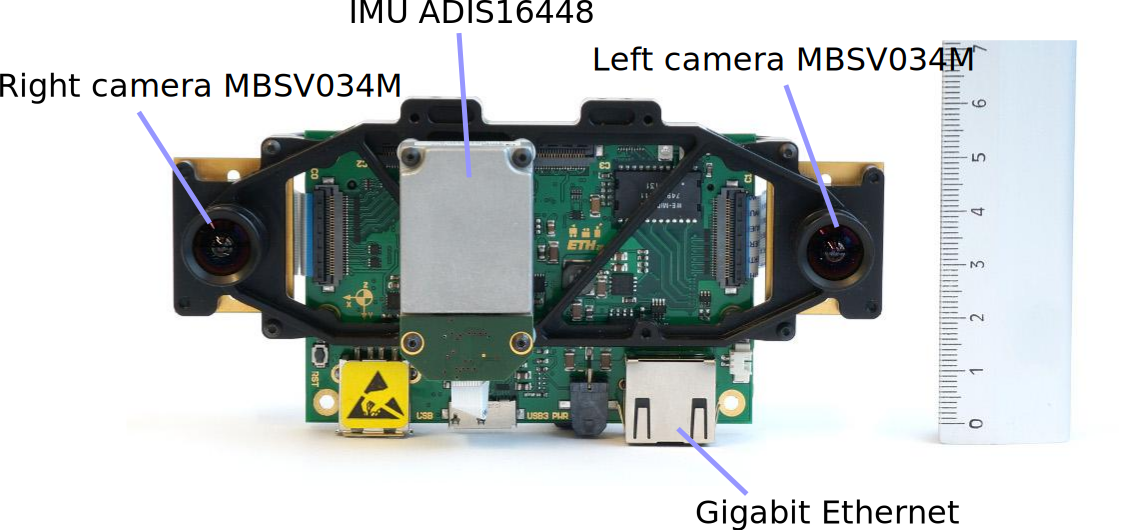
\includegraphics[width=\textwidth]{figures/introduction/vi_sensor_details.pdf}
\end{figure}
\end{frame}

\begin{frame}{Our system}
\begin{figure}[!htb]
\centering
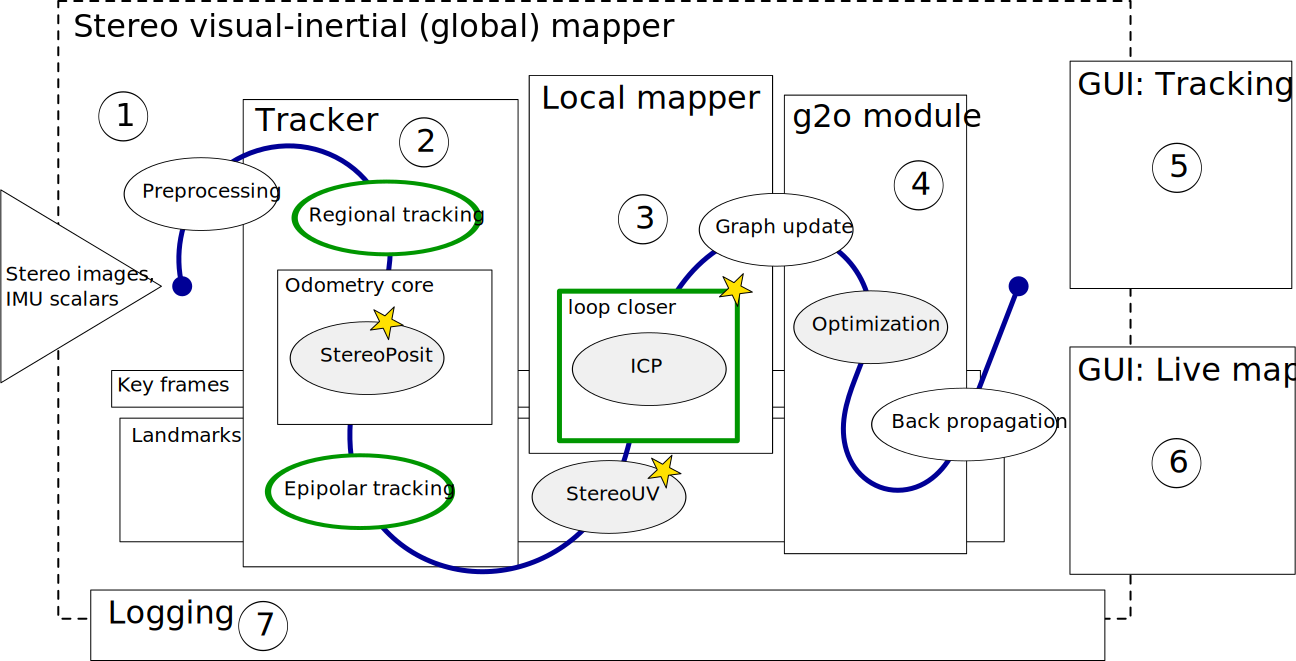
\includegraphics[width=\textwidth]{figures/approach_softwaredesign/pipeline.pdf}
\end{figure}
Contributions: StereoPosit, StereoUV, Loop closure detection
\end{frame}

%\begin{frame}{First steps}
%\begin{figure}[!htb]
%\centering
%\includegraphics[width=\textwidth]{figures/introduction/first_steps.pdf}
%\end{figure}
%Many simplifications:
%\begin{itemize}
%\item Indoor datasets with slow steady movement
%\item Odometry by Alberto\texttrademark
%\item Minimal range and disturbance
%\end{itemize}
%\end{frame}

%\begin{frame}{Least squares state optimization}
%\begin{itemize}
%\item StereoUV $\to$ Landmark position\\\vspace{5pt}
%\hspace{10pt}State: Positions $\mathbf{x}(x,y,z)$\\
%\hspace{10pt}Measurements: Projections $p_L,p_R$\\
%\vspace{10pt}
%\item StereoPosit $\to$ Odometry\\\vspace{5pt}
%\hspace{10pt}State: Transformation $T_{21}(R,\mathbf{t})$\\
%\hspace{10pt}Measurements: Positions $\mathbf{x}$, projections $p_L,p_R$\\
%\vspace{10pt}
%\item ICP (Besl et al) $\to$ Loop closures\\\vspace{5pt}
%\hspace{10pt}State: Transformation $T_{BA}$\\
%\hspace{10pt}Measurements: Positions $\mathbf{x}_A,\mathbf{x}_B$\\
%\vspace{10pt}
%\end{itemize}
%\end{frame}

%\begin{frame}{Tracking: Complete pipeline}
%\begin{figure}[!htb]
%\centering
%\includegraphics[width=\textwidth]{figures/approach_tracking/pipeline_tracking_module.pdf}
%\end{figure}
%\begin{itemize}
%\item Multi-stage tracking approach
%\item IMU integration (odometry)
%\item Contribution: StereoPosit optimization
%\end{itemize}
%\end{frame}

\begin{frame}{Tracking: Regional tracking
%\footfullcite{Shi, J., Tomasi, C.: Good features to track. In: Computer Vision and Pattern Recognition, 1994. Proceedings CVPR’94., 1994 IEEE Computer Society Conference}
\footfullcite{Calonder, M., Lepetit, V., Strecha, C., Fua, P.: Brief: Binary robust independent elementary features. Computer Vision-ECCV 2010}}
\begin{figure}[!htb]
\centering
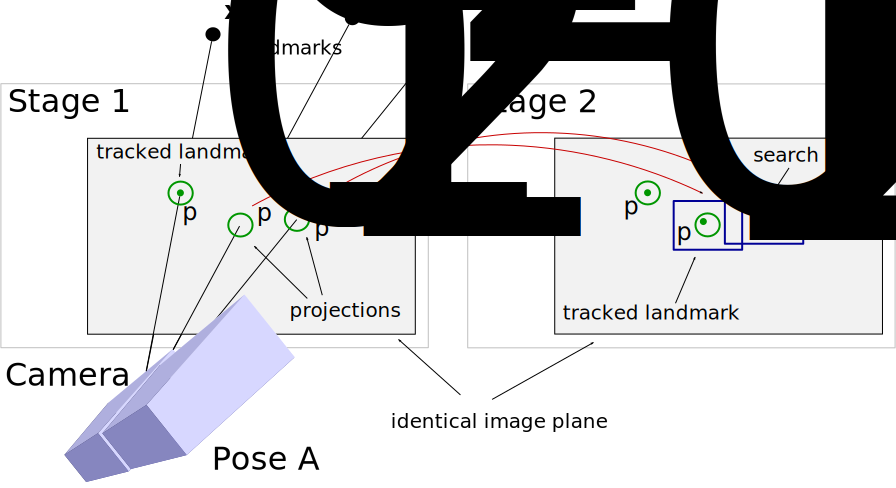
\includegraphics[width=\textwidth]{figures/approach_tracking/concept_regional_tracking.pdf}
\end{figure}
\end{frame}

\begin{frame}{Tracking: Epipolar tracking
\footfullcite{Richard, Hartley; Andrew, Z.: Multiple View Geometry in Computer Vision. Cambridge University Press (March 2004)}}
\begin{figure}[!htb]
\centering
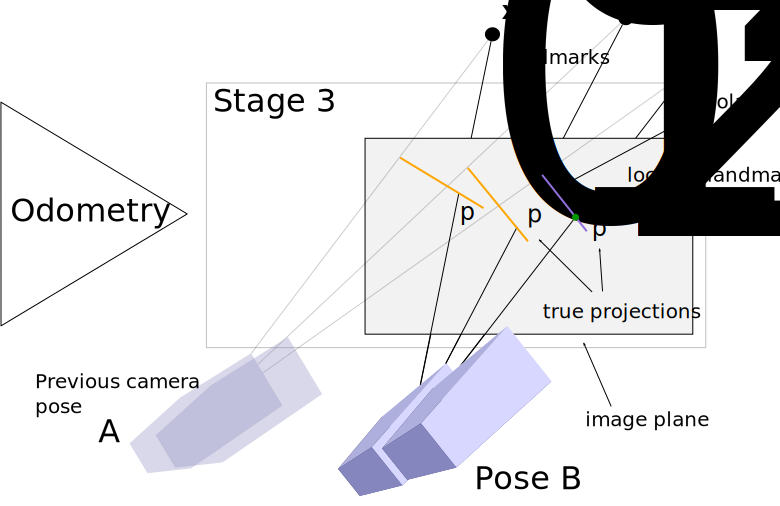
\includegraphics[width=0.75\textwidth]{figures/approach_tracking/concept_epipolar_tracking.pdf}
\end{figure}
In action: \href{run:/home/n551jw/Documents/presentation_ma/aula_magna.ogv}{\textcolor{blue}{Aula Magna}}
\end{frame}

%\begin{frame}{Loop closing: Problem statement}
%\begin{figure}[!htb]
%\centering
%\includegraphics[width=\textwidth]{figures/approach_loopclosing/problem_scenario.pdf}
%\end{figure}
%Measures to solve this problem:
%\begin{itemize}
%\item Detection of loop closures (déjà vu moment)
%\item Determine spatial relation between closures
%\end{itemize}
%\end{frame}

\begin{frame}{Loop closing: Our approach}
\begin{figure}[!htb]
\centering
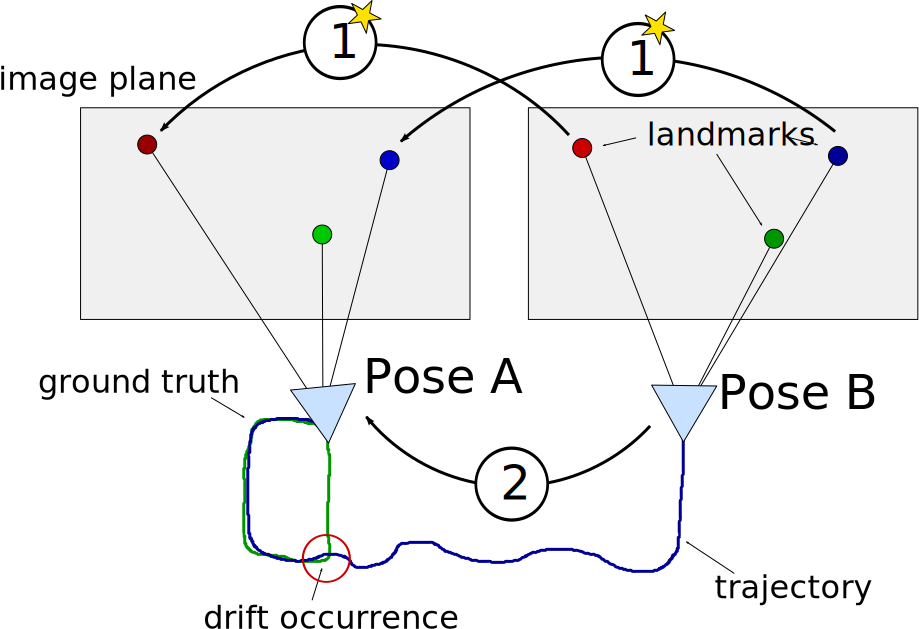
\includegraphics[width=0.7\textwidth]{figures/approach_loopclosing/loop_closing.pdf}
\end{figure}
\begin{itemize}
\item Step 1: Find matching landmarks (Contribution)
\item Step 2: Compute spatial relation: ICP
\footfullcite{Besl, P.J., McKay, N.D.: Method for registration of 3-D shapes. Proc. SPIE 1611 (1992)}
\hfill \href{run:/home/n551jw/Documents/presentation_ma/aula_magna.ogv}{\textcolor{blue}{Aula Magna}}
\end{itemize}
\end{frame}

%\begin{frame}
%\frametitle{System in action}
%Hand-held dataset: \href{run:/home/n551jw/Documents/presentation_ma/aula_magna.ogv}{Aula Magna}
%\begin{figure}[!htb]
%\centering
%\includegraphics[width=\textwidth]{figures/movie_aula_magna.png}
%\end{figure}
%\end{frame}

\begin{frame}{Data acquisition
\footfullcite{Geiger, A., Lenz, P., Urtasun, R.: Are we ready for autonomous driving? the KITTI
vision benchmark suite (CVPR 2012)}}
\begin{figure}[!htb]
\centering
\includegraphics[width=0.7\textwidth]{figures/results/data_acquisition.pdf}
\end{figure}
\end{frame}

\begin{frame}
\frametitle{Results: Hand-held}
\begin{figure}[!htb]
\centering
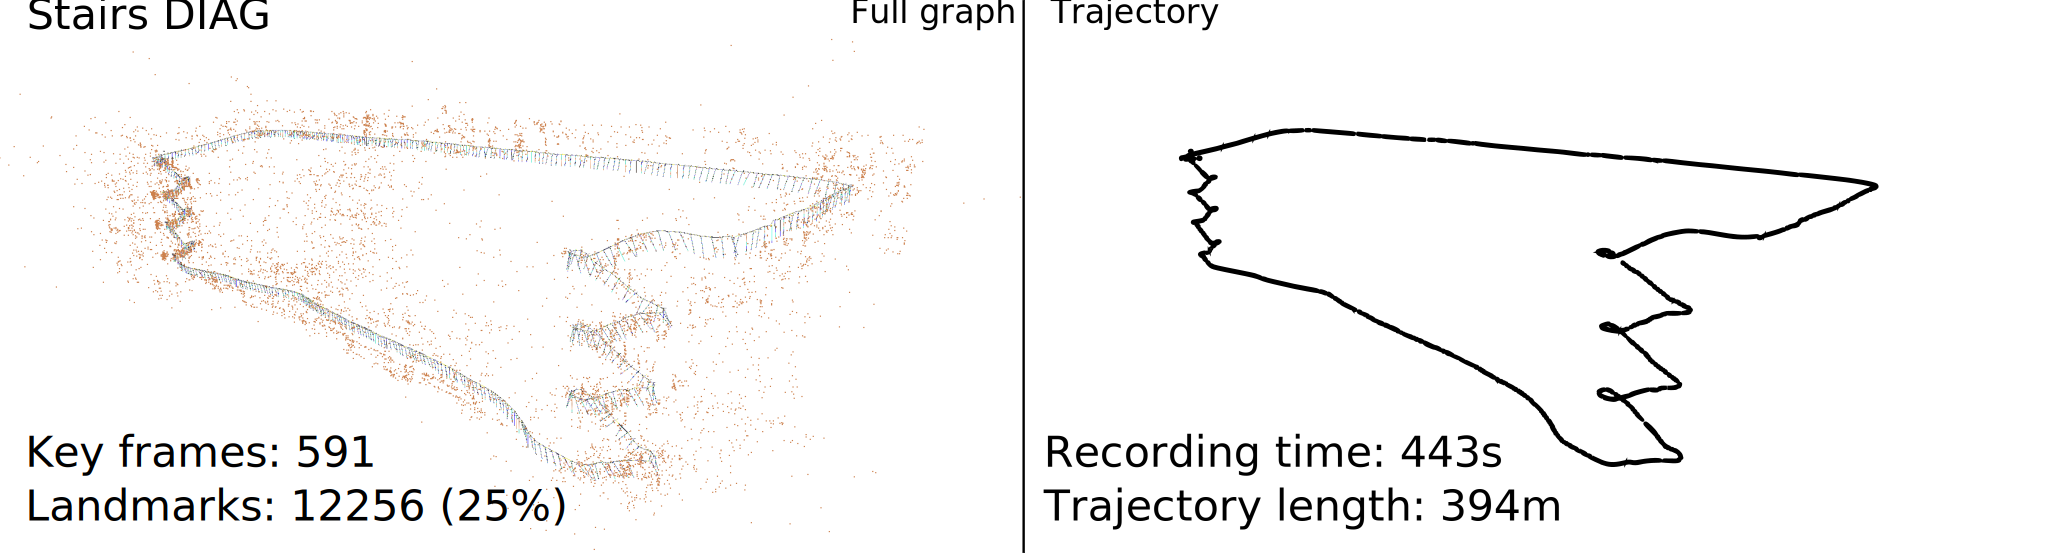
\includegraphics[width=\textwidth]{figures/results/stairs_combined.pdf}
\end{figure}
\begin{figure}[!htb]
\centering
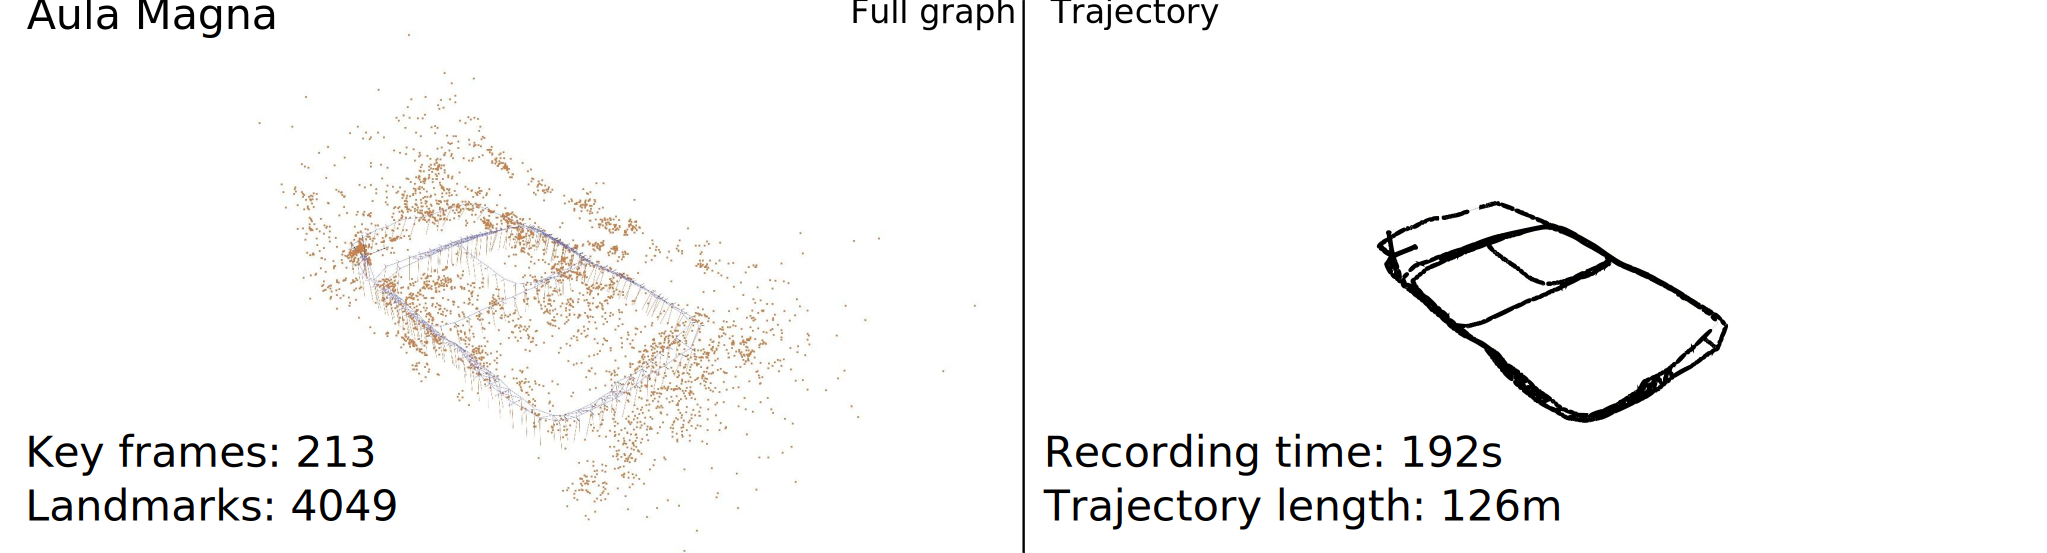
\includegraphics[width=\textwidth]{figures/results/aula_magna.pdf}
\end{figure}
\end{frame}

\begin{frame}
\frametitle{Results: Bike}
\begin{figure}[!htb]
\centering
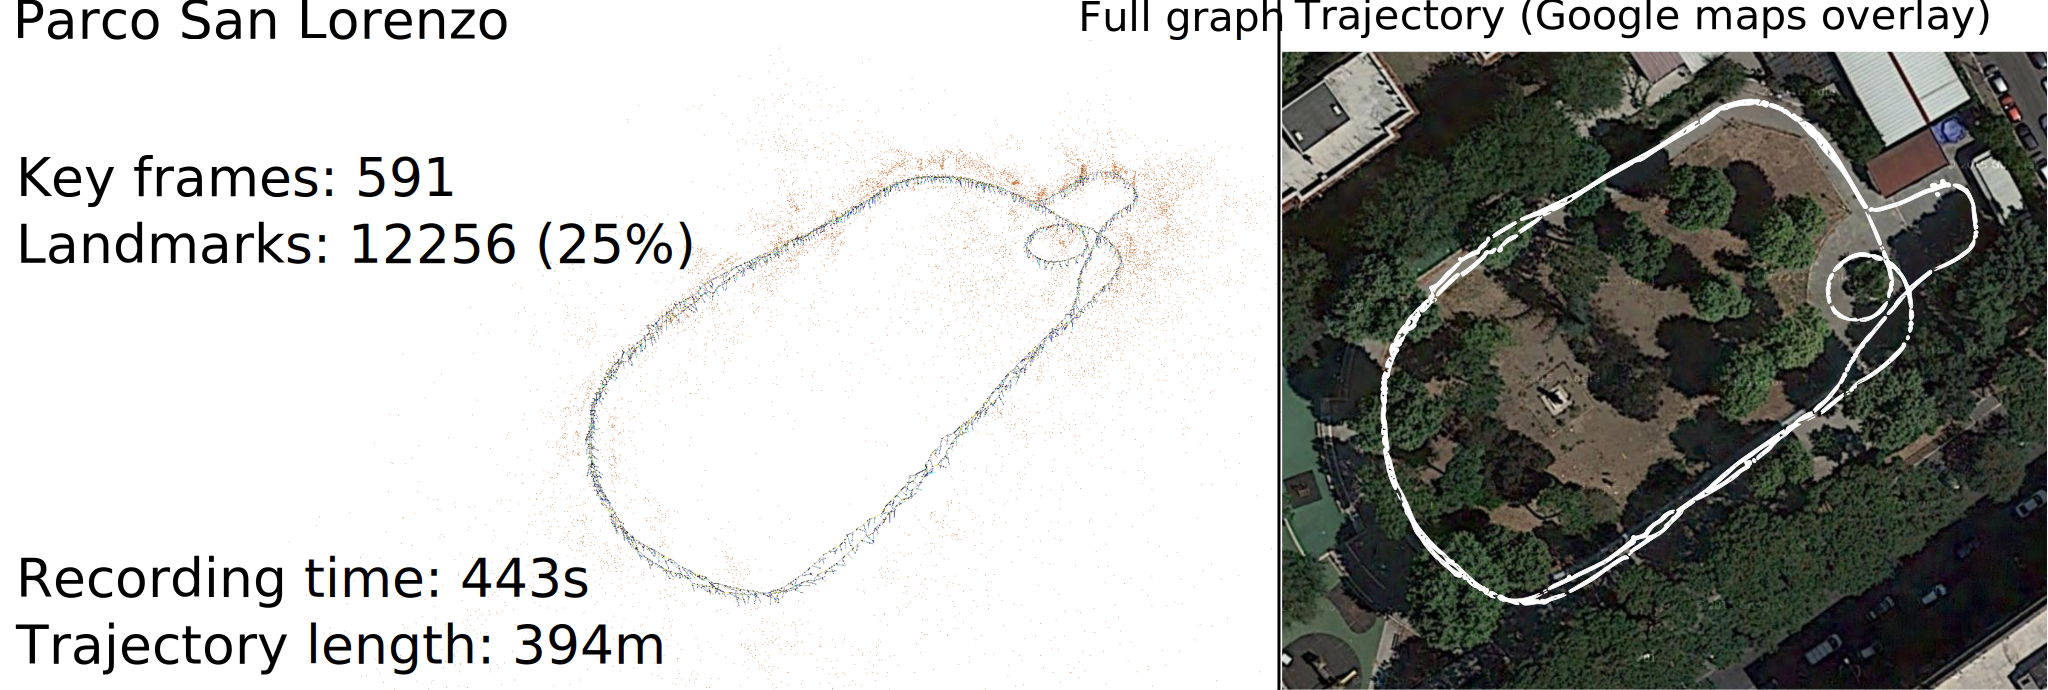
\includegraphics[width=0.8\textwidth]{figures/results/san_lorenzo_parco.pdf}
\end{figure}
\begin{figure}[!htb]
\centering
\includegraphics[width=0.8\textwidth]{figures/results/san_lorenzo_street.pdf}
\end{figure}
\end{frame}

\begin{frame}
\frametitle{Results: KITTI odometry benchmark (without IMU)}
Trajectory overlay: \hfill Errors (KITTI standard): \hspace{25pt}
\begin{figure}[!htb]
\centering
\includegraphics[width=0.49\textwidth]{figures/results/00.pdf}\hspace{10pt}
\begin{subfigure}[b]{0.46\textwidth}
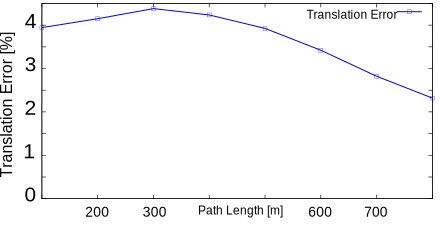
\includegraphics[width=\textwidth]{figures/results/00_tl.pdf}\\
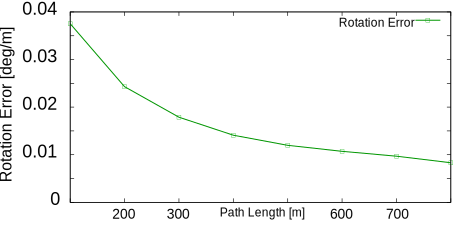
\includegraphics[width=\textwidth]{figures/results/00_rl.pdf}
\end{subfigure}
\end{figure}
Total trajectory length: 3722m
\end{frame}

%\begin{frame}{Trajectory error}
%\begin{figure}[!htb]
%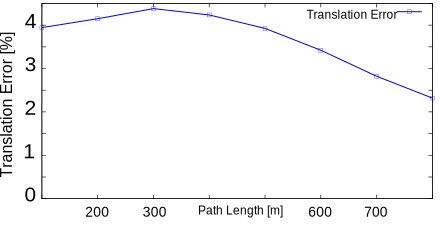
\includegraphics[width=0.65\textwidth]{figures/results/00_tl.pdf}\\
%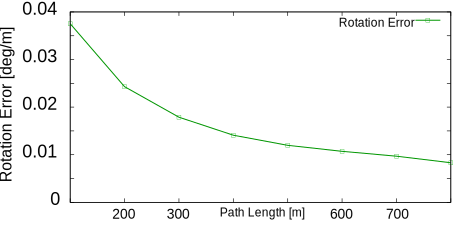
\includegraphics[width=0.65\textwidth]{figures/results/00_rl.pdf}
%\end{figure}
%\end{frame}

\begin{frame}{Conclusions and remarks}
Final system:
\begin{itemize}
\item Outstanding robustness
\item High accuracy (Map overlays, 1-5\% KITTI error)
\item Strong, independent odometry (KITTI)
\item Modularity (Multithreading)
\end{itemize}
\vspace{10pt}
Future work:
\begin{itemize}
\item Filter integration
\footfullcite{Forster, C., Carlone, L., Dellaert, F., Scaramuzza, D.: IMU Preintegration on Manifold
for Efficient Visual-Inertial Maximum-a-Posteriori Estimation. (RSS 2015)} (IMU)
\item Improved feature handling
\footfullcite{Rublee, E., Rabaud, V., Konolige, K., Bradski, G.: ORB: an efficient alternative to
SIFT or SURF. (ICCV 2011)}
\item Improved graph optimization
\footfullcite{Grisetti, Giorgio, Rainer Kuemmerle, and Kai Ni. Robust optimization of factor graphs by using condensed measurements. (IROS 2012)}
\end{itemize}
\end{frame}

{
\setbeamertemplate{footline}{} 
\usebackgroundtemplate{
\includegraphics[width=\paperwidth]{figures/titlepage.pdf}}
\begin{frame}
\vspace{-70pt}
\center{\Huge{\textcolor{white}{\inserttitle}}}\\
\vspace{20pt}
\begin{minipage}{1.07\textwidth}
\textcolor{white}{\hfill\small{\insertauthor}}\\
\textcolor{white}{\hfill\small{Supervisor: Prof. Dr. Giorgio Grisetti}}
\end{minipage}
\vspace{10pt}\\
\hspace{-28pt}\textcolor{white}{\small{\insertdate}}
\end{frame}
}

\end{document}
